
\documentclass{article} % Don't change this

\usepackage{tabularx} % extra features for tabular environment
\usepackage{amsmath}  % improve math presentation
\usepackage{graphicx} % takes care of graphic including machinery
\usepackage[margin=1.25in,letterpaper]{geometry} % decreases margins
\usepackage{cite} % takes care of citations
\usepackage{subfigure}
\usepackage{float}    % For tables and other floats
\usepackage[final]{hyperref} % adds hyper links inside the generated pdf file
\usepackage{listings}
\usepackage[framed,numbered,autolinebreaks,useliterate]{mcode}
\usepackage{lipsum}
\hypersetup{
	colorlinks=true,       % false: boxed links; true: colored links
	linkcolor=blue,        % color of internal links
	citecolor=blue,        % color of links to bibliography
	filecolor=magenta,     % color of file links
	urlcolor=blue         
}
\newcommand{\blah}{blah blah blah \dots}



\setlength{\marginparwidth}{3.4cm}

% NEW COUNTERS
\newcounter{points}
\setcounter{points}{100}
\newcounter{spelling}
\newcounter{usage}
\newcounter{units}
\newcounter{other}
\newcounter{source}
\newcounter{concept}
\newcounter{missing}
\newcounter{math}

% COMMANDS
%\newcommand{\raisa}[2]{\colorbox{Yellow}{#1} \todo{#2}}
\newcommand{\arbitrary}[2]{\todo{#1 #2} \addtocounter{points}{#2} \addtocounter{other}{#2}}
\newcommand{\english}{\todo{LANGUAGE (-1)} \addtocounter{points}{-1}
\addtocounter{usage}{-1}}
\newcommand{\units}{\todo{UNITS (-1)} \addtocounter{points}{-1}
\addtocounter{units}{-1}}
\newcommand{\spelling}{\todo{SPELLING and GRAMMAR (-1)} \addtocounter{points}{-1}
\addtocounter{spelling}{-1}}
\newcommand{\source}{\todo{SOURCE(S) (-2)} \addtocounter{points}{-2}
\addtocounter{source}{-2}}
\newcommand{\concept}{\todo{CONCEPT (-2)} \addtocounter{points}{-2}
\addtocounter{concept}{-2}}
\newcommand{\missing}[2]{\todo{MISSING CONTENT (#1) #2} \addtocounter{points}{#1}
\addtocounter{missing}{#1}}
\newcommand{\maths}{\todo{MATH (-1)} \addtocounter{points}{-1}
\addtocounter{math}{-1}}

\newcommand{\summary}[1]{
\begin{mdframed}[nobreak=true]
\begin{minipage}{\textwidth}
\vspace{0.5cm}
\begin{center}
\Large{Grade Summary} \hrule 
\end{center} \vspace{0.5cm}
General Comments: #1

\vspace{0.5cm}
Possible Points \dotfill 100 \\
Points Lost (Spelling and Grammar) \dotfill \thespelling \\
Points Lost (Language) \dotfill \theusage \\
Points Lost (Units) \dotfill \theunits \\
Points Lost (Math) \dotfill \themath \\
Points Lost (Sources) \dotfill \thesource \\
Points Lost (Concept) \dotfill \theconcept \\
Points Lost (Missing Content) \dotfill \themissing \\
Other \dotfill \theother \\[0.5cm]
\begin{center}
\large{\textbf{Grade:} \fbox{\thepoints}}
\end{center}
\end{minipage}
\end{mdframed}}

%#########################################################

%To use symbols for footnotes
\renewcommand*{\thefootnote}{\fnsymbol{footnote}}
%To change footnotes back to numbers uncomment the following line
%\renewcommand*{\thefootnote}{\arabic{footnote}}

% Enable this command to adjust line spacing for inline math equations.
% \everymath{\displaystyle}

% _______ _____ _______ _      ______ 
%|__   __|_   _|__   __| |    |  ____|
%   | |    | |    | |  | |    | |__   
%   | |    | |    | |  | |    |  __|  
%   | |   _| |_   | |  | |____| |____ 
%   |_|  |_____|  |_|  |______|______|
%%%%%%%%%%%%%%%%%%%%%%%%%%%%%%%%%%%%%%%

\title{
\normalfont \normalsize 
\textsc{Rutgers University \\ 
Summer Research Program} \\
[10pt] 
\rule{\linewidth}{0.5pt} \\[6pt] 
\huge Implementation of Gaussian Process  \\
\rule{\linewidth}{2pt}  \\[10pt]
}
\author{Han Liu}
\date{\normalsize \today}

\begin{document}

\maketitle



\section{Introduction}
For my understanding of Gaussian Process (GP), GP is a function that maps a set of random variables to another set of random variables, and there are two quantatives to specify the process: mean and covariance matrix. Genrally, the mean is 0 (if it's not zero, we can transform it into 0), therefore, to uniquely describe a GP of multiply variables, we only need to specify its covariance matrix. This process can be easily achieved by defining a kernel function, which needs to satisfy the following property:
\begin{itemize}
	\item Symmetric and positive definite
	\item Satisfy the general meaning of covariance 
\end{itemize}
Take squared exponential kernel for example, which is :
\begin{equation}\label{eq1}
k(x,x^{'})=exp(\frac{-(x-x^{'})^2}{2\eta^2})
\end{equation}
When the $x$ and $x^{'}$ are close, $k$ is approaching to 1, but if they are far from each other, $k$ is quite small, so they satisfy the general meaning of covariance.\\

I think GP's biggest advantage compared to other model is that it can get a explicit expression, by which we can predict the confidence of the data, and can optimize the process to a more efficient level (such as BBMM parallel computation). Instead, traditional prediction model (neural network, etc) is more like a black box, we don't know the explicit relationship between the input and output, which sets obstacles for optimization.\\

In the following section, I have tried to implement the general process of GP and during the trianing process, I used two methods to implement it in python. Finally, I have compared my results with Sk-learn. 


\section{Methodology}
I divide the general process of GP into training and testing. In the training process, we need to get hyperparameters of chosen kernel function by using existed data. In the testing process, we need to use trained model to predict the output.
\subsection{Training Process}
The goal of training process is to maximize the marginal likelihood function. In this example, I choose squared exponential kernel given in Eq. \ref{eq1}. Specifically, we denote the input as $x$, output as $y$, the covariance matrix between $x$ is $K$, the variance matrix of input data is $\sigma^2I_{00}$. After some calculations (I have omitted here), we can get:
\begin{equation}
p({y|\sum})\sim N(0,\sum+\sigma^2I_{00})
\end{equation}
Let $K$ denotes $\sum+\sigma^2I_{00}$, by expanding it into Gaussian expression:
\begin{equation}
logp({y|K})=-\frac{1}{2}log((2\pi)^k|K|)-\frac{1}{2}y^T{K}^{-1}y
\end{equation}
In order to achieve that, I apply the stochastic gradient descent. The gradient of marginal likelihood function is as following:
\begin{equation}
\frac{\partial}{\partial \theta_j}logp(y|X,\theta)=\frac{1}{2}y^{T}K^{-1}\frac{\partial K}{\partial \theta_j}K^{-1}y-\frac{1}{2}tr(K^{-1}\frac{\partial K}{\partial \theta_j})
=\frac{1}{2}tr((\alpha\alpha^T)-K^{-1}\frac{\partial K}{\partial \theta_j})
\end{equation}
Where $\alpha=K^{-1}y$. In the following, I have tried two different methods, but only succeeded in the last one. \\
In the first method, I tried to use simple gradient descent to implement the training, specifically, the hyperparameter of kernel function is updated through the following ways: 
\begin{equation}
\theta=\theta-\frac{\partial}{\partial \theta_j}logp(y|X,\theta)
\end{equation}
The code is as following:
\begin{lstlisting}
def Get_Grad(x_sample,y_sample,std,alpha,gamma):
cov_sample=RBF_ker(x_sample,x_sample,gamma,False)
cov_grad=RBF_ker(x_sample,x_sample,gamma,True)
K = np.diag(np.array(std) ** 2 )+cov_sample
L=cholesky(K, lower=True)               # Use cholesky decomposition to get inverse
alpha = cho_solve((L, True), y_sample)
K_inverse = cho_solve((L, True), np.eye(K.shape[0]))
grad_gamma=-1/2*np.trace(np.dot(np.dot(alpha,alpha.T)-K_inverse,cov_grad))
return grad_gamma

def GP_model_train(x_sample,y_sample,std,alpha):
gamma=0.05                                #Initialize the parameter of kernal
grad_gamma = Get_Grad(x_sample, y_sample, std, alpha, gamma)
count=0
while grad_gamma < 10 ** (-5) or count > 500:
gamma = gamma - alpha * grad_gamma  # gradient descent
grad_gamma = Get_Grad(x_sample, y_sample, std, alpha, gamma)
count += 1
return gamma
\end{lstlisting}
However, I met the problem of gradient explosion: $\theta$ does not converge. I found that this simple optimization strategy can not handle this complex function. To utilize complex optimization strategy, I decided to use tensorflow. Specifically, I set the target function as $-logp(y|K)$, and I have calculated the relationship between target function and input data, the code is as following:

\begin{lstlisting}
def GP_model_train(x_sam,y_sam,Std):
sess = tf.Session()
gamma = tf.Variable(tf.random_normal([1, 1], stddev=1, seed=1))
length=len(x_sam)

x = tf.placeholder(tf.float32, shape=(1,length), name='x-input')
y_ = tf.placeholder(tf.float32, shape=(1, length), name='y-input')
std=tf.placeholder(tf.float32, shape=(1, length), name='std-input')

cov=tf.exp(tf.divide(tf.square(tf.transpose(x) - x),-2*tf.square(gamma)))

K = tf.add(tf.matrix_diag(tf.square(std)),cov)
K=tf.reshape(K,(length,length))
K_deter=tf.matrix_determinant(K)
K_inv=tf.matrix_inverse(K)

#Left Side
cons=tf.pow(tf.multiply(2.0,tf.constant(m.pi)),length)             
cons_1=tf.multiply(cons,K_deter)
cons_2=tf.log(cons_1)
left=tf.multiply(0.5,cons_2)
#Right side
y_=tf.reshape(y_,(1,length))
rig_1=tf.matmul(y_,K_inv)
rig_2=tf.matmul(rig_1,tf.transpose(y_))
right=tf.multiply(0.5,rig_2)

loss=tf.add(left,right)

train_step = tf.train.AdamOptimizer(0.001).minimize(loss)
#dataset
X = np.array(x_sam).reshape(1,length)
Y = np.array(y_sam).reshape(1,length)
STD = np.array(Std).reshape(1,length)

with tf.Session() as sess:
init_op = tf.global_variables_initializer()
sess.run(init_op)
STEPS = 5000
count=0
for i in range(STEPS):
sess.run(train_step, feed_dict={x: X, y_: Y,std:STD})
return gamma.eval()[0][0]

\end{lstlisting}	
	 After reviewing some of the literature, I found that the optimized function $logp({y|K})$ is non-convex, which may lead that the optimized function converges to a local minimum, so I tried to initialize the hyperparameter randomly.
\subsection{Testing Process}
To predict (or test) a new input, we need to get its posterior probability. By the property of the joint Gaussian distribution, we can get the posterior probability:
\begin{equation}
p(\hat{y}|{y})\sim N(\sum_{10}K^{-1}y,\sum_{11}-\sum_{10}K^{-1}\sum_{01})
\end{equation}
Where $\sum_{10}$ is the covariance matrix between test sequence and train sequence. After getting mean and covariance matrix, it is easy to write the expression:
\begin{equation}
f(x_1,x_2,...,x_k)=\frac{1}{\sqrt{(2\pi)^k|\sum|}} exp(-\frac{1}{2}(x-u)^T\sum^{-1}(x-u)
\end{equation}
\section{Experiment}
In this section, I have done two sets of tests, including comparation test and stability test.\\

For the comparation part, I have compared my method with GPR function in sk-learn library. I use the same function $y=xsin(x)$ to be predicted with same input. The results are as following:
\begin{figure}[H]
	\centering
	\subfigure[My Method]{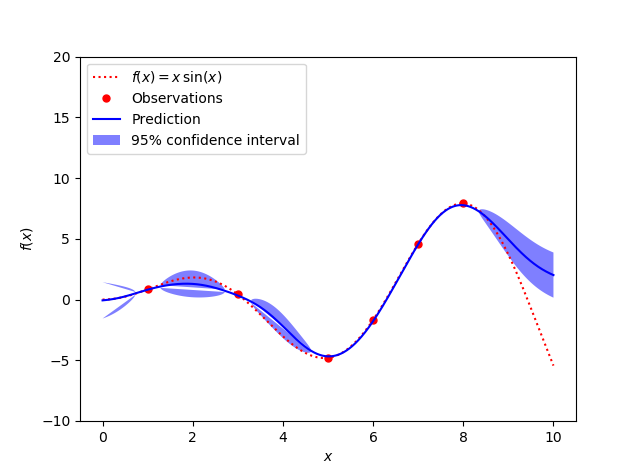
\includegraphics[width=2.7in]{my_test}}
	\subfigure[Sk-learn]{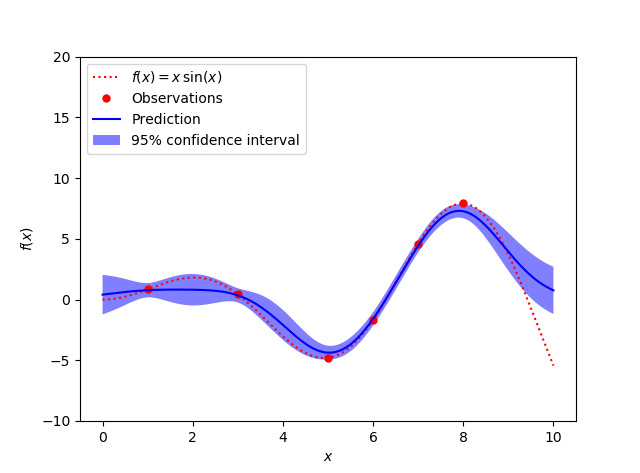
\includegraphics[width=2.7in]{skl}}
	\caption{Comparison of Two Implementations}
	\label{fig1}
\end{figure}
For the stability tests, I want to know how stable the predicted value is, so I have produce seven sets of predicted value based on a same input, I also show the 95\% confidence level, the results are as following:
 \begin{figure}[H]
	\begin{center}
		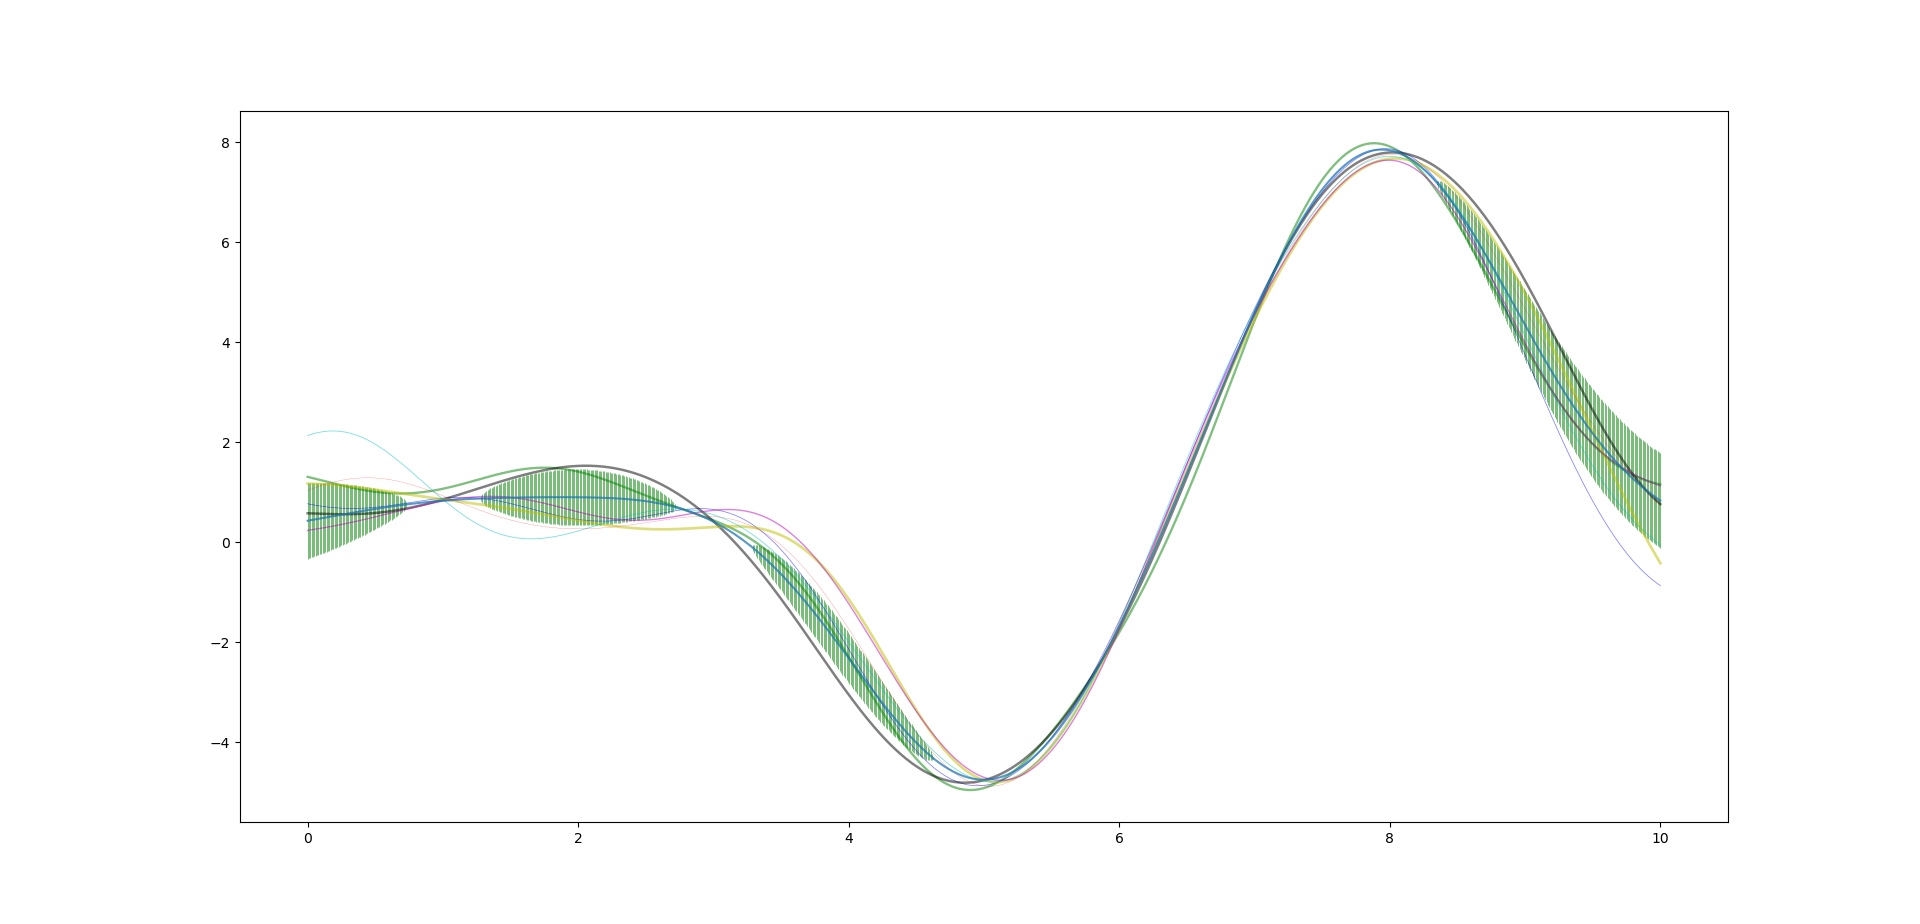
\includegraphics[width=0.85\textwidth]{stability}
	\end{center}
	\caption{Results of Seven Sets of Predicted Values }
	\label{fig2}
\end{figure}

\section{Discussion}
From Figure \ref{fig1}, it is easy to see two methods have similar pattern, also, they agree with the truth value $f(x)=xsin(x)$. It is also worthy mentioning that in the interval with observation value, the predicted line fits the original function very well, however, it does not fit very well outside the interval. This is due to the defficiency of input value.\\

From Figure \ref{fig2}, it is easy to see the eight lines are quite close to each other, also, the variance is small, which proves the stability of prediction.\\


\end{document} % NOTHING AFTER THIS LINE IS PART OF THE DOCUMENT
